\documentclass[12pt,a4paper]{article}
\topmargin -1.6cm
\addtolength{\textheight}{4cm}
\textwidth  15.5cm

\leftmargin      5mm
\rightmargin     5mm
\oddsidemargin   5mm
\evensidemargin  5mm

\usepackage{hyperref}
\usepackage{polski}
\usepackage[utf8]{inputenc}
\usepackage{graphicx}
\usepackage{units}
\usepackage{sty/style}

\projekt{Modelowanie obiektu manipulatora 2R (EDDA)}
\autor{Marcin Bober, 249426}
\przedmiot{Projekt specjalnościowy ARR}
\prowadzacy{Dr inż. Mirela Kaczmarek}

\begin{document}
\pdfpageheight   297mm
\pdfpagewidth    210mm

\StronaTytulowa
\SpisTresci

\pagebreak

\section{Badany obiekt}

\section{Algorytm Qui Dorsey'a}
  \subsection{Opis} %(algorytmu i obiektu)
  \subsection{Wyniki} %tabelka - zmiany nastaw a rząd błędu

  \begin{table}[h!]
    \centering
    \begin{tabular}{ r | r | c | c }
      P & D & $e_1$ & $e_2$  \\ 
      \hline
      10 & 1 & $10^{-1}$ & $10^{-1}$ \\  
      100 & 10 & $10^{-1}$ & $10^{-2}$ \\  
      1000 & 100 & $10^{-2}$ & $10^{-3}$ \\  
      10000 & 1000 & $10^{-3}$ & $10^{-4}$ \\  
      100000 & 10000 & $10^{-4}$ & $10^{-5}$ \\  
      1000000 & 100000 & $10^{-1}$ & $10^{-1}$
    \end{tabular}
    \caption{Table to test captions and labels.}
    \label{table:1}
  \end{table}

  \begin{figure}[ht]
    \centering
    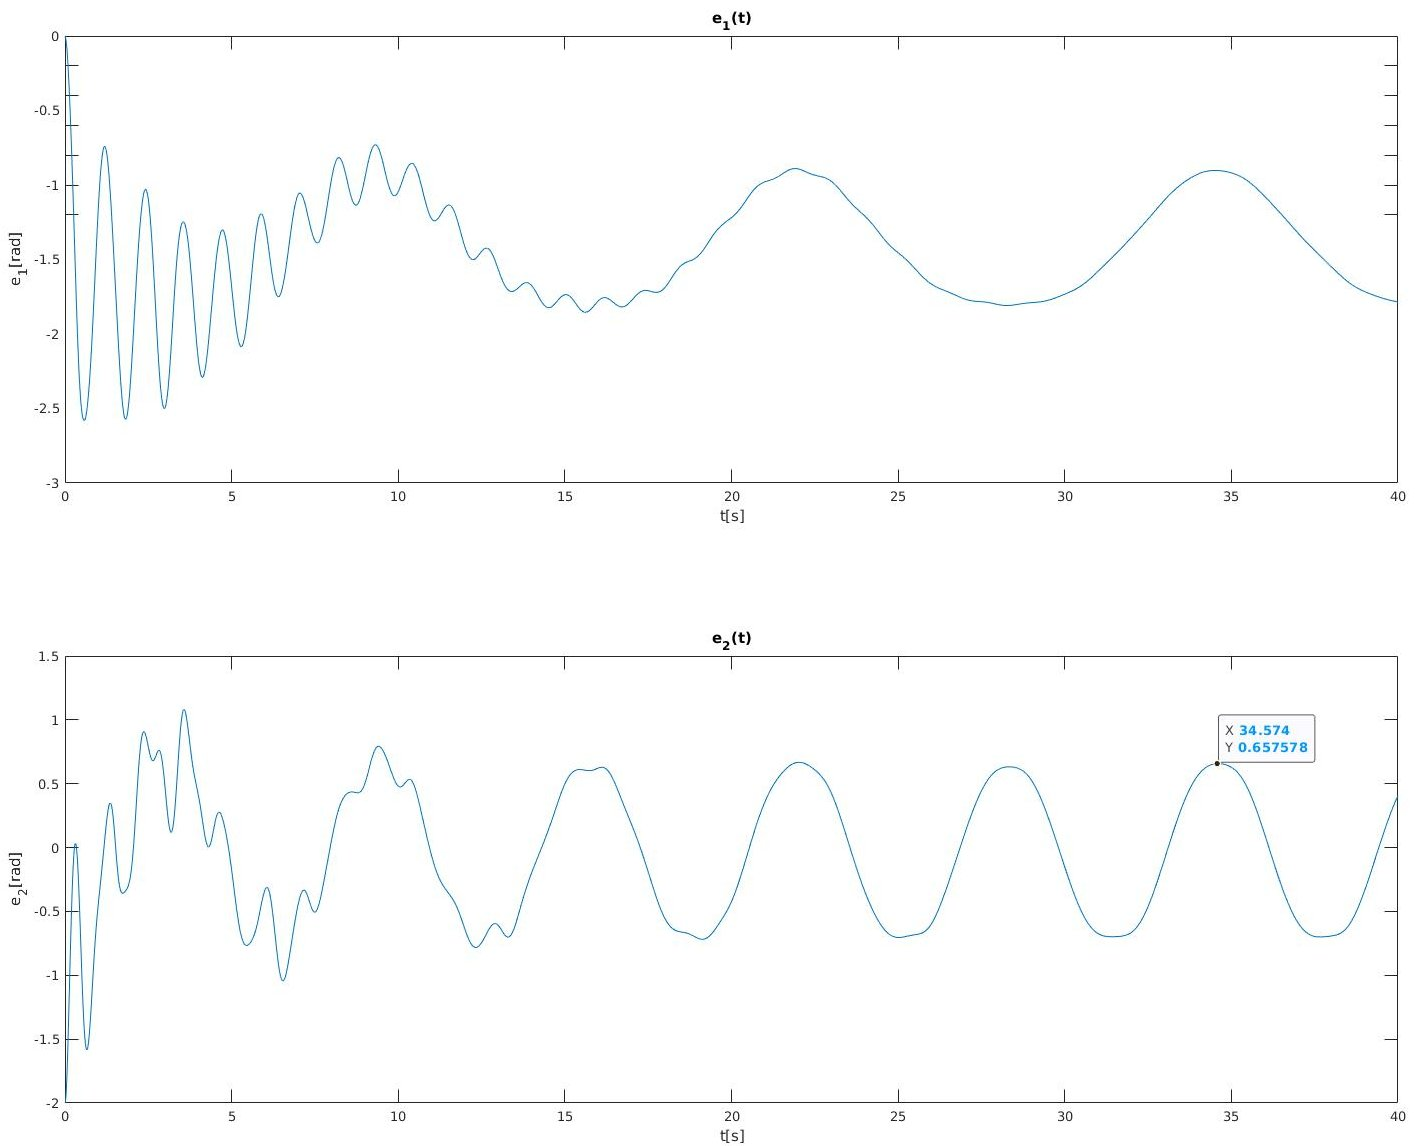
\includegraphics[width=1\textwidth]{figures/qui10.jpg}
    \caption{KP = 10, KD = 1}
  \end{figure}

  \begin{figure}[ht]
    \centering
    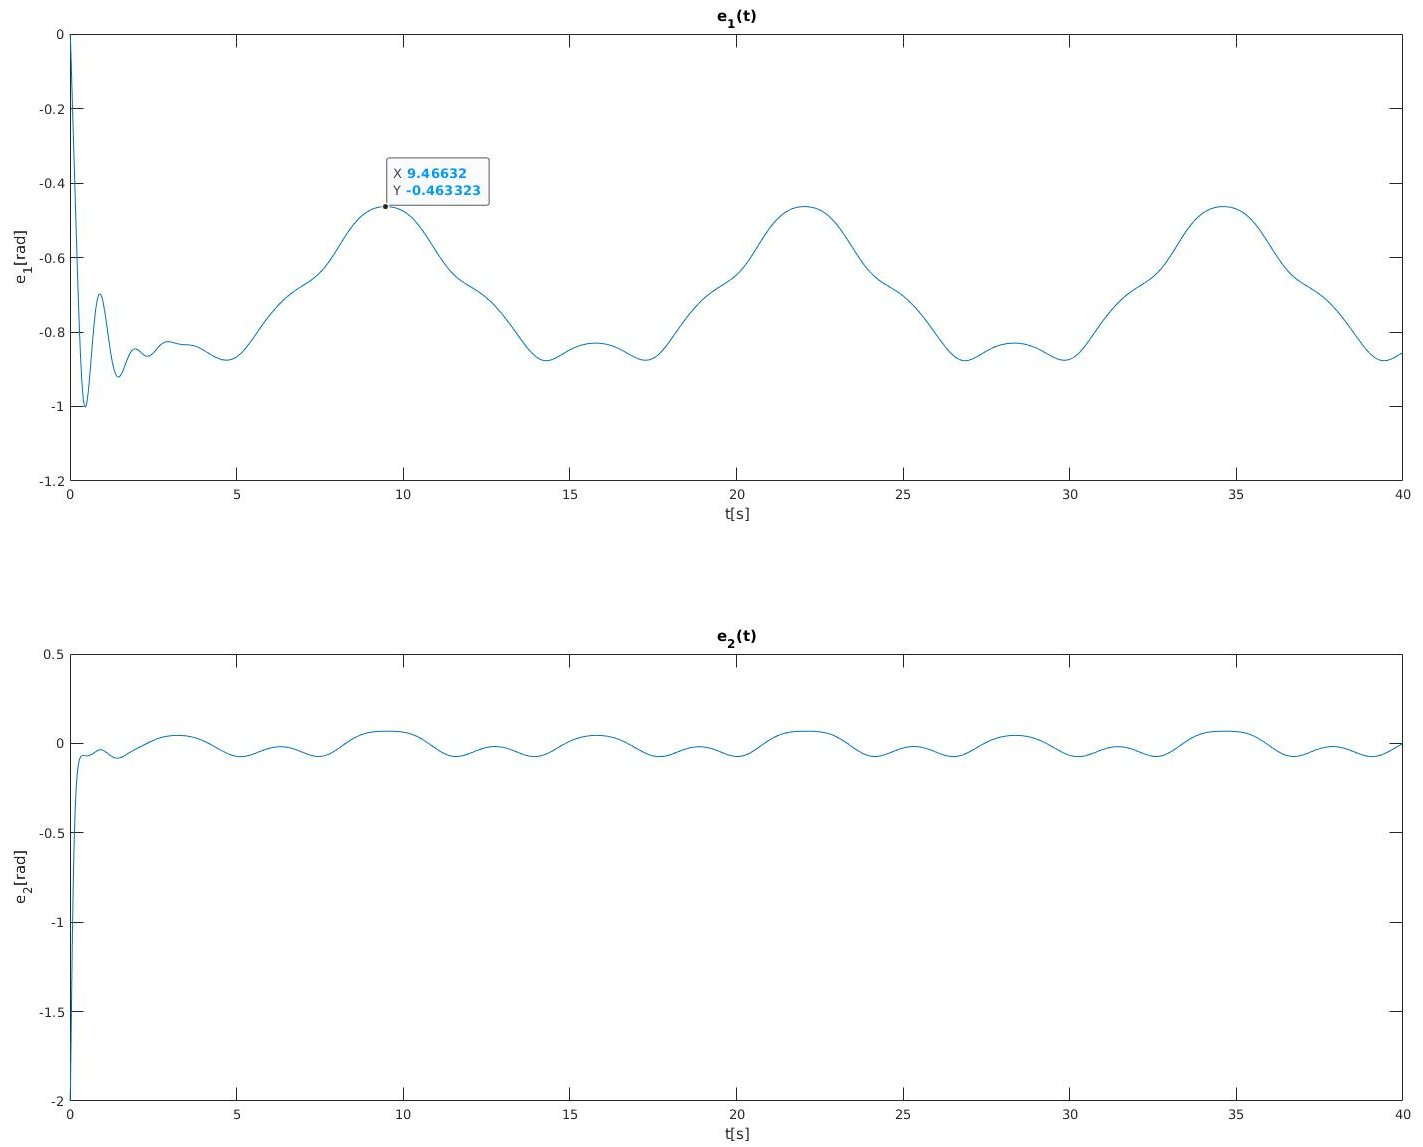
\includegraphics[width=1\textwidth]{figures/qui100.jpg}
    \caption{KP = 100, KD = 10}
  \end{figure}

  \begin{figure}[ht]
    \centering
    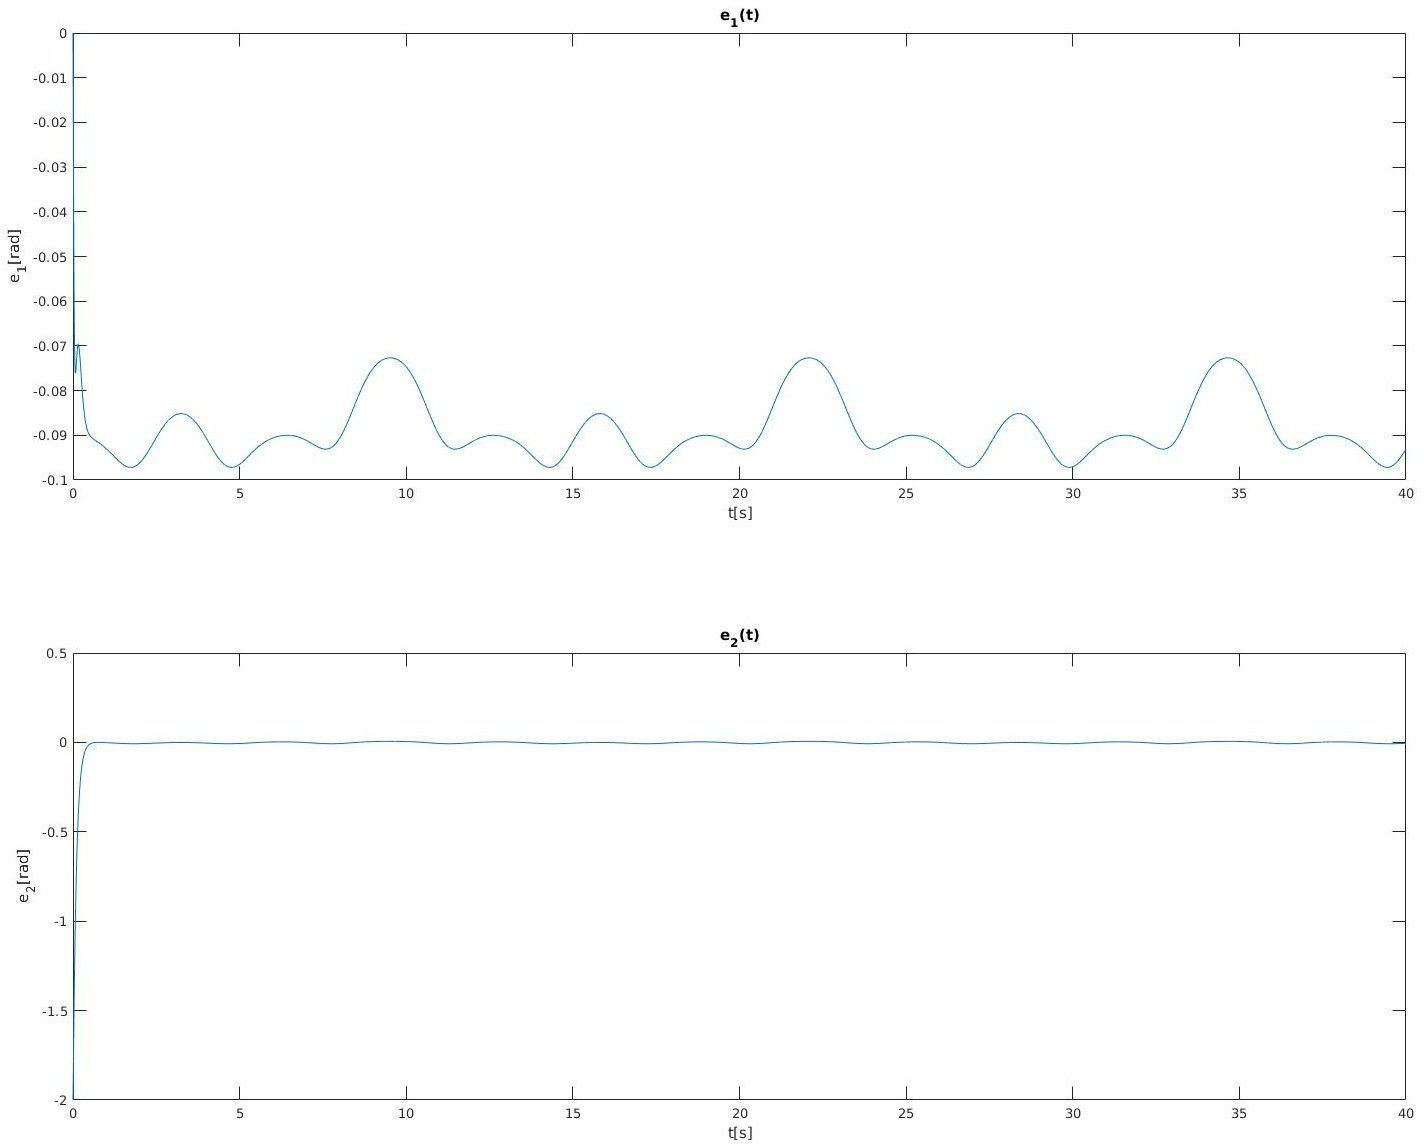
\includegraphics[width=1\textwidth]{figures/qui1000.jpg}
    \caption{KP = 1000, KD = 100}
  \end{figure}

  \begin{figure}[ht]
    \centering
    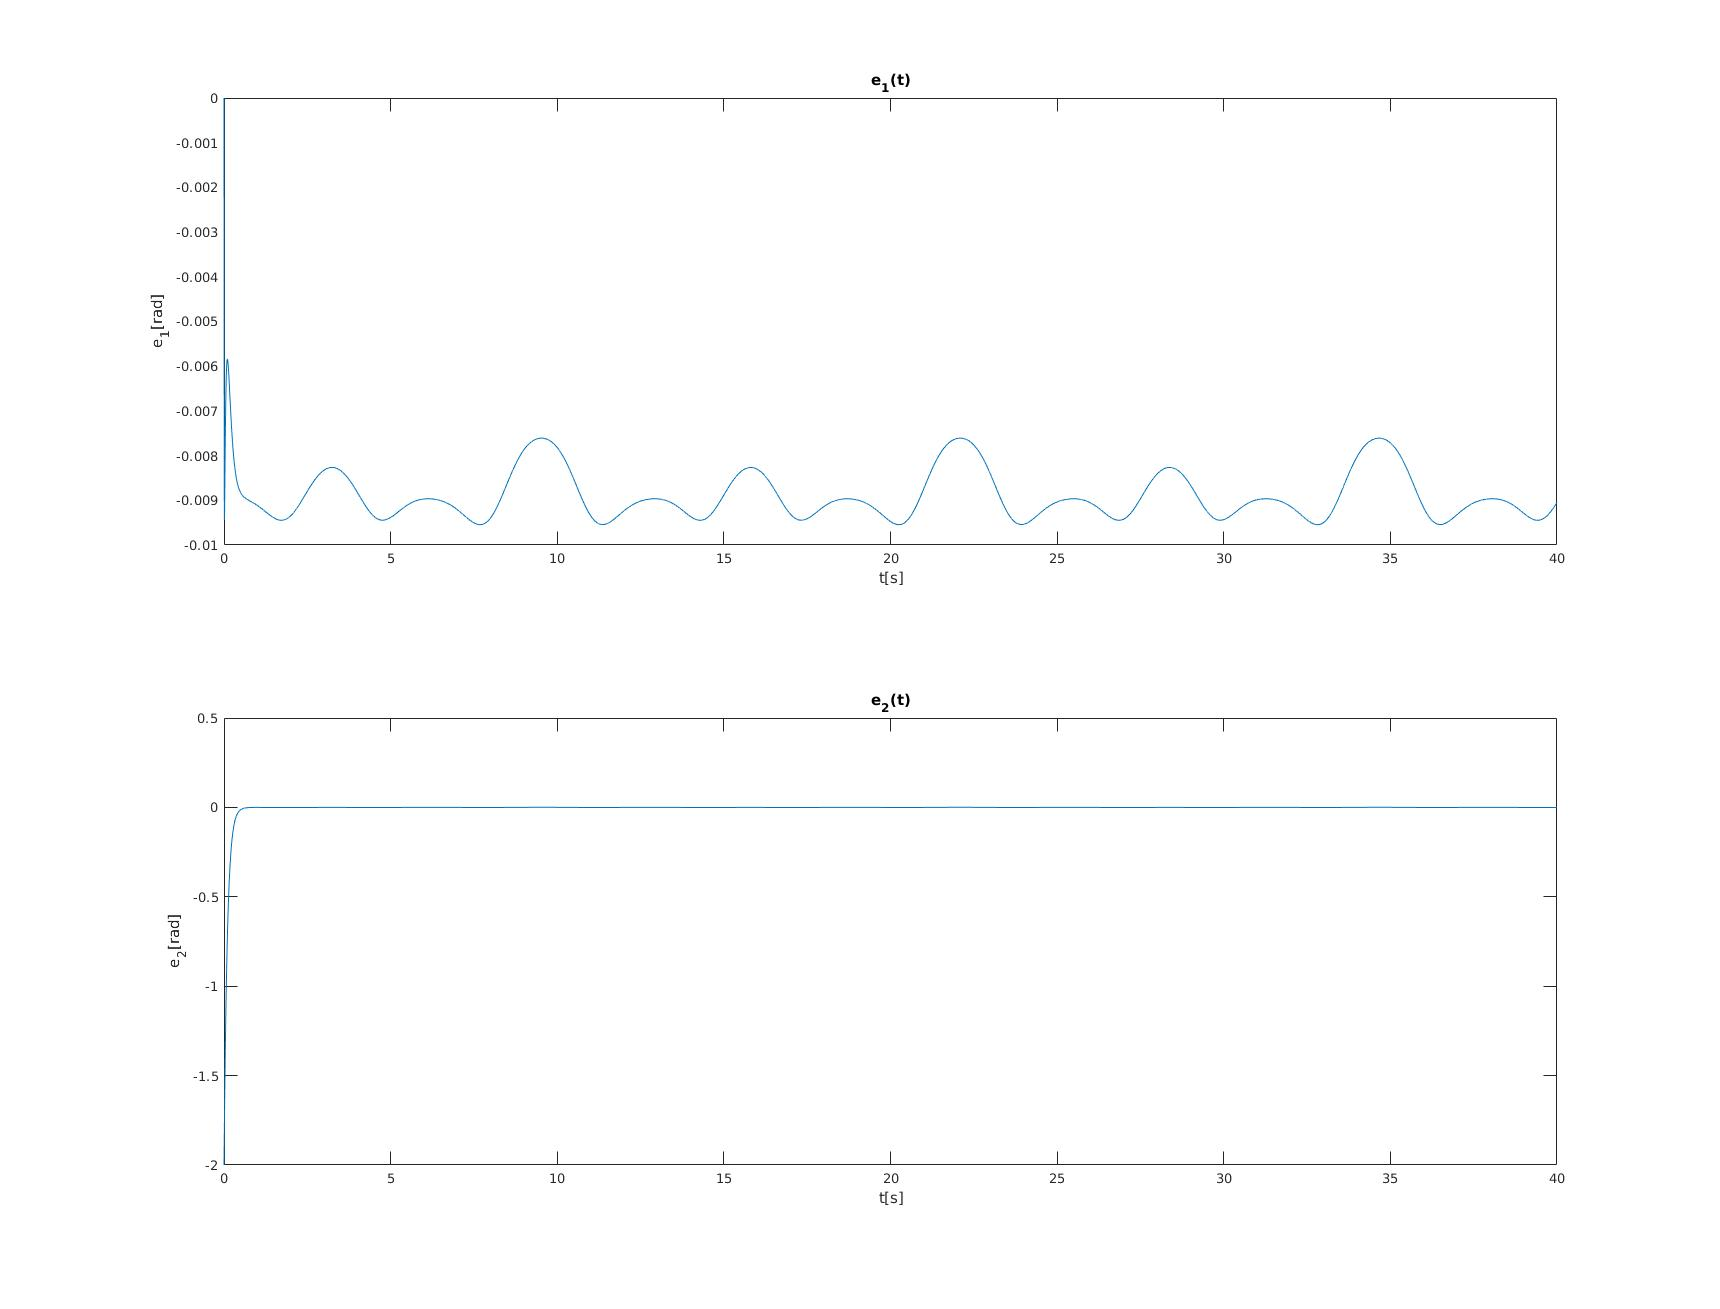
\includegraphics[width=1\textwidth]{figures/qui10000.jpg}
    \caption{KP = 10000, KD = 1000}
  \end{figure}

  \begin{figure}[ht]
    \centering
    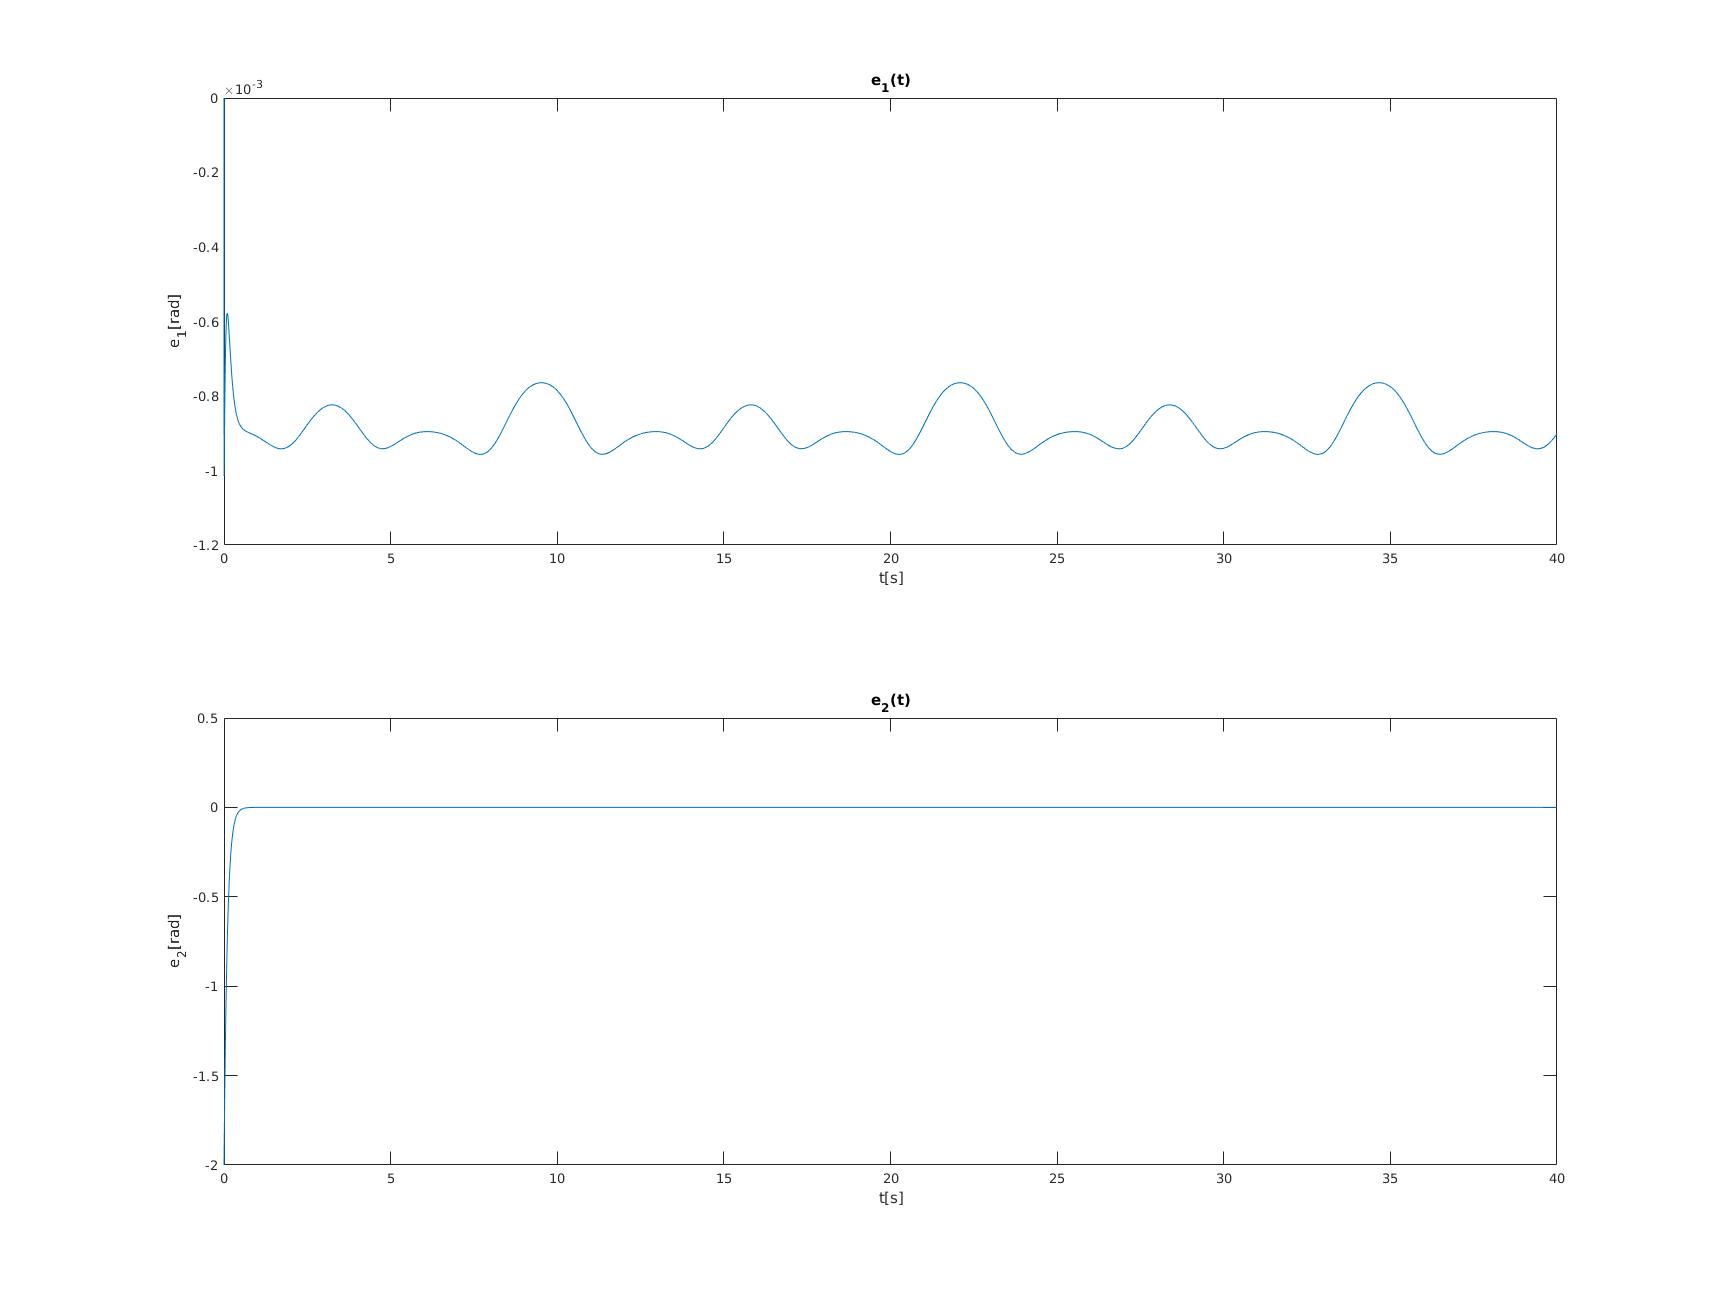
\includegraphics[width=1\textwidth]{figures/qui100000.jpg}
    \caption{KP = 100000, KD = 10000}
  \end{figure}

  % \begin{figure}[ht]
  %   \centering
  %   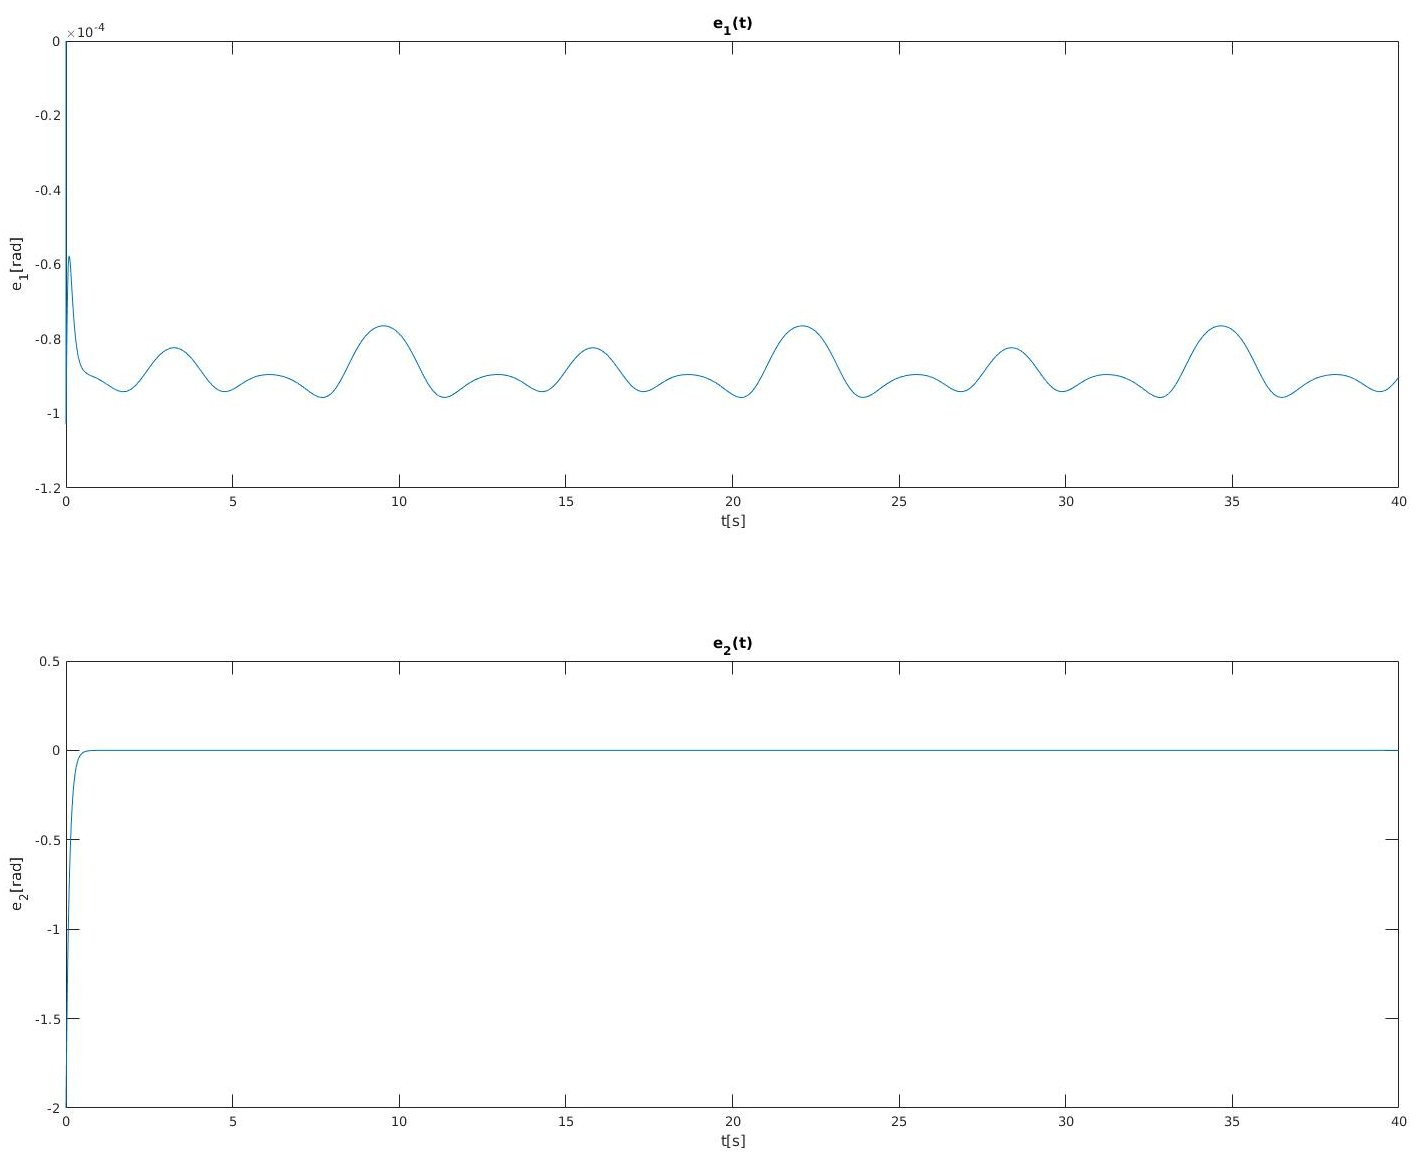
\includegraphics[width=1\textwidth]{figures/qui1000000.jpg}
  %   \caption{KP = 1000000, KD = 100000}
  % \end{figure}

  \subsection{Wnioski}

\section{Algorytm dokładnej linearyzacji}
  \subsection{Opis} %(algorytmu i obiektu)
  \subsection{Wyniki} %tabelka - zmiany nastaw a rząd błędu
  \subsection{Wnioski}

\section{Podsumowanie}



%   \begin{figure}[H]
%     \centering
%     \includegraphics[width=1\textwidth]{img/img3.png}
%     \caption{Macierze transformacji}
%   \end{figure}

%   \section{Wyznacz kinematykę manipulatora w SE(3)}
  
%   \begin{figure}[H]
%     \centering
%     \includegraphics[width=1\textwidth]{img/img2.png}
%     \caption{Kinematyka manipulatora}
%   \end{figure}

%   \begin{figure}[H]
%     \centering
%     \includegraphics[width=1\textwidth]{img/img4.png}
%     \caption{Kinematyka manipulatora}
%   \end{figure}

\end{document}